\documentclass[article,A4,12pt]{llncs}
\usepackage[T1]{fontenc}
\usepackage{amsmath}
\usepackage{amssymb}
\usepackage{amsfonts}
\usepackage{mathrsfs, bm}

\usepackage{graphicx}
\usepackage{tabularx}
\usepackage{subfig}
\usepackage{epsf,times}
\usepackage{color}
\usepackage{wrapfig}
\usepackage{cases}
\usepackage{multicol}

\usepackage[T1]{fontenc}
%\newcommand{\tmname}[1]{\textsc{#1}}
%\newcommand{\tmop}[1]{\ensuremath{\operatorname{#1}}}
%\newcommand{\tmsamp}[1]{\textsf{#1}}
%\newcommand{\tmtextsc}[1]{{\scshape{#1}}}
%\newcommand{\tmtextsl}[1]{{\slshape{#1}}}
%\newcommand{\tmtexttt}[1]{{\ttfamily{#1}}}

\leftmargin=0.0cm
\oddsidemargin=0.5cm
\evensidemargin=0.5cm
\topmargin=0cm
\textwidth=16.0cm
%\textheight=21.5cm
\textheight=20.0cm
\pagestyle{plain}
\setlength{\columnsep}{20pt}

\def\m{\mathbf{m}}
\def\H{\mathbf{H}}
\def\E{\mathbf{E}}
\newcommand{\vepsi}{{\varepsilon}}
\def\hnorm#1#2{\vert\,#1\,\vert_{#2}}
\newcommand{\R}{{\mathbb R}}
\newcommand{\Sph}{{\mathbb S}}
\def\x{\mathbf{x}}
\def\hvec{\overline{\mathbf{h}}}
\def\evec{\overline{\mathbf{e}}}

\newcommand{ \etal}{\mbox{\emph{et al. }}}

\newcommand\vect[1]{\mbf{#1}}
\newcommand{\mbf}[1]{\mbox{\boldmath$#1$}} 
\newcommand{\RC}[1]{#1 $\times$ #1 $\times$ #1}
\def\um{$\mu$m}
\def\C{$^{\circ}\mathrm{C}$}

\newcommand{\Rmnum}[1]{\expandafter\@slowromancap\romannumeral #1@}

% DEFINITION OF CUSTOM FONT SIZE
\newcommand{\customfontA}{\fontsize{50}{55}\selectfont}
\newcommand{\customfontB}{\fontsize{14.4}{20}\selectfont}
\newcommand{\customfontC}{\fontsize{30}{35}\selectfont}

\DeclareMathAlphabet{\mathpzc}{OT1}{pzc}{m}{it}

\def\clovek#1{\noindent\bgroup\vbox{\noindent#1}\egroup\vskip1em}

% TO INPUT BACKGROUND IMAGE
\usepackage{eso-pic}
\newcommand\BackgroundPic{
\put(0,0){
\parbox[b][\paperheight]{\paperwidth}{
\vfill
\centering
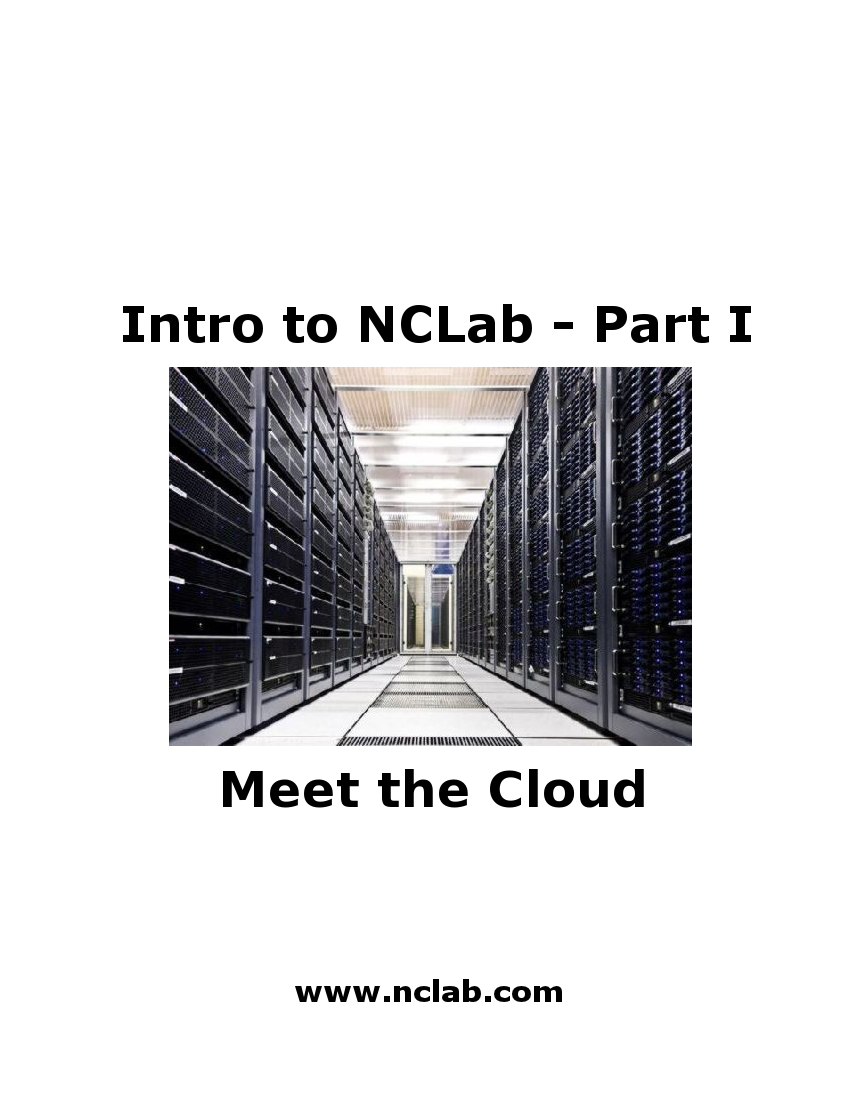
\includegraphics[width=\paperwidth,height=\paperheight]{img/intro-frontpage.png}
%\includegraphics[width=\paperwidth,height=\paperheight]{img/background.jpg}
\vfill
}}}

\begin{document}

% INPUTTING BACKGROUND IMAGE
\AddToShipoutPicture{\BackgroundPic}
\vbox{}
\pagestyle{empty}
\newpage
\textwidth=15.5cm
\ClearShipoutPicture
\newpage

%%%%%%%%%%%%%%%%%%%%%%%%%%%%%%%%%%%%%%%%%%%%%%%%%%%%%%%%%%%%%%%%%%%%%%%%%

\section*{}
\small
\input ../common/aboutnclab.tex

\subsection*{Acknowledgement}
This publication was created with the help of numerous freely 
available web resources and tutorials related to Python, Scipy,
Numpy, Pylab, Matplotlib, Sympy and other projects.

\normalsize

\newpage
%{\ }
\setcounter{tocdepth}{2}
\tableofcontents
%\pagestyle{plain}

\newpage

\pagestyle{plain}
\setcounter{page}{1}

%%%%%%%%%%%%%%%%%%%%%%%%%%%%%%%%%%%%%%%%%%%%%%%%%%%%%%%%%%%%%%%%%%%%%%%%%

\section{What is the {\em Cloud}?}

Using cloud computing or cloud computers sounds like a rocket science, but it is not,
and it really changes things for the better. Chances are that you are using 
it already, without even knowing. For example, if you are using free email services of Gmail, 
Hotmail, Yahoo or another such provider, then your data are stored on the cloud. If you are 
using free Google docs to acces your Word or Excel files from anywhere, you are using the cloud
as well. 

\subsection{Basic Facts}

In the IT sense of the word, and with a bit of simplification, the {\em cloud} 
is a pool of interconnected computers. They come in different sizes depending on the provider - 
large cloud facilities have millions of computers but some companies are running 
their own private clouds with relatively few ones. The computers in large clouds
are not very similar to your desktop PC -- they are stripped off many unnecessary 
things, compacted, and interconnected into a powerful grid. Their processors 
typically contain multiple {\em computing cores} that can share the same memory.
Such {\em multicore processors} are much more efficient compared to (clusters 
of) PCs with equivalent number of cores.

The main advantage of the cloud is its {\em elasticity}. Upon your request, the
provider will assemble for you an {\em instance} with the parameters that 
you need. An instance means a computer with given parameters (number of processors, 
hard disk size, memory). An instance is created within a minute or so, and the user can upgrade 
or downgrade it dynamically, depending on the actual needs. After the instance is 
no longer needed, it is dissolved and the same hardware is used to build instances 
for other users. The following is a realistic example of how such instances may 
look like (just the name of the provider was omitted):\\

\begin{center}
\begin{tabular}{|l|l|l|l|}
\hline
{\bf Small instance} & 1.7 GB of memory & 1 core & 160 GB hard disk \\
\hline
{\bf Medium instance} & 7.5 GB of memory & 4 cores & 850 GB hard disk \\
\hline
{\bf Large instance} & 15 GB of memory & 8 cores & 1690 GB hard disk \\
\hline
\end{tabular}
\end{center}

\vspace{4mm}
\noindent
Importantly - these three instances are created by grouping the same resources together 
in different ways. 
It is quite interesting to look at the prices:

\begin{center}
\begin{tabular}{|l|l|}
\hline
{\bf Small instance} &	\$0.085 per hour\\
\hline
{\bf Medium instance}&	\$0.34 per hour	\\
\hline
{\bf Large instance}&	\$0.68 per hour\\
\hline
\end{tabular}
\end{center}

\vspace{4mm}
\noindent
With such low prices, literally anyone has now access to 
a powerful computer -- that otherwise would cost many thousands of dollars -- 
for just cents per hour. This brings new wonderful opportunities to ordinary users
and educators.

\subsection{Software as a Service (SaaS)}

Another big change that cloud computing brings is in how software is handled. 
Traditionally, one would buy a software in a big box with a small CD in it, 
and install it on one's computer. This model is now being challenged by a new 
approach called {\em Software as a Service (SaaS)}. The user does not have 
to own a copy of the software physically. Instead, the software is running 
on a remote server and accessed by users over the Internet. Typically, paying 
for the access is much less expensive compared to buying the software. If you like,
think about it like watching a movie on Netflix vs. buying a DVD. 

\subsection{Access from Mobile Platforms}

Last but not least, since the software is running on the cloud, the user's hardware 
does not matter so much anymore. The only really important things is to be able to 
run a web browser and access the Internet. This can be done on anything between smart 
phones, tablets, netbooks, laptops, and desktop computers. 

\subsection{Some Myths}

Very often, cloud computing is mentioned in the context of large 
computations in science, engineering, finance, and other fields. This is because there are many 
cloud providers and they need to show off. But in reality, the clouds are mostly
busy processing small tasks of ordinary users. In that case, you may say, a standard 
office PC should be enough. Not exactly. Once you are not in your office, for example
while traveling, it is difficult to reach your office PC and do things as usual. 
The cloud changes that -- it allows you to access your data 
from everywhere, any time. Once you get used to it, there is no way back. 

\subsection{NCLab and K-12 Education}

NCLab is a web-based framework that provides 
instant access to programming, web design, math, physics, 3D CAD design, computer
modeling, and scientific computing. You do not have to install it or care about 
anything -- NCLab 
is automatically available in any classroom that has Internet access. In 
contrast to traditional educational software products, 
users can access their accounts and work from anywhere and at any time.
Students can start a problem at school, finish the rest at home, and notify 
the instructor about the completion with one mouse click. Most importantly, 
however, NCLab invites K-12 teachers and students to discover new exciting 
areas that were out of their reach before.

%%%%%%%%%%%%%%%%%%%%%%%%%%%%%%%%%%%%%%%%%%%%%%%%%%%%%%%%%%%%%%%%%%%%%%%%%
\newpage

\section{Getting Started}

In order to explore NCLab, first visit its home page {\tt http://nclab.com}.
Under the logo you will see a slide show representing selected activities 
offered by NCLab. The Cloud Monitor, located under the slide show, displays 
the current load on the core cluster. By default, NCLab runs on six nodes 
with a total of 200 computing cores, and has approximately 200 GB of memory 
available for immediate use. These parameters are scaled dynamically 
as needed. 

\begin{figure}[!ht]
\begin{center}
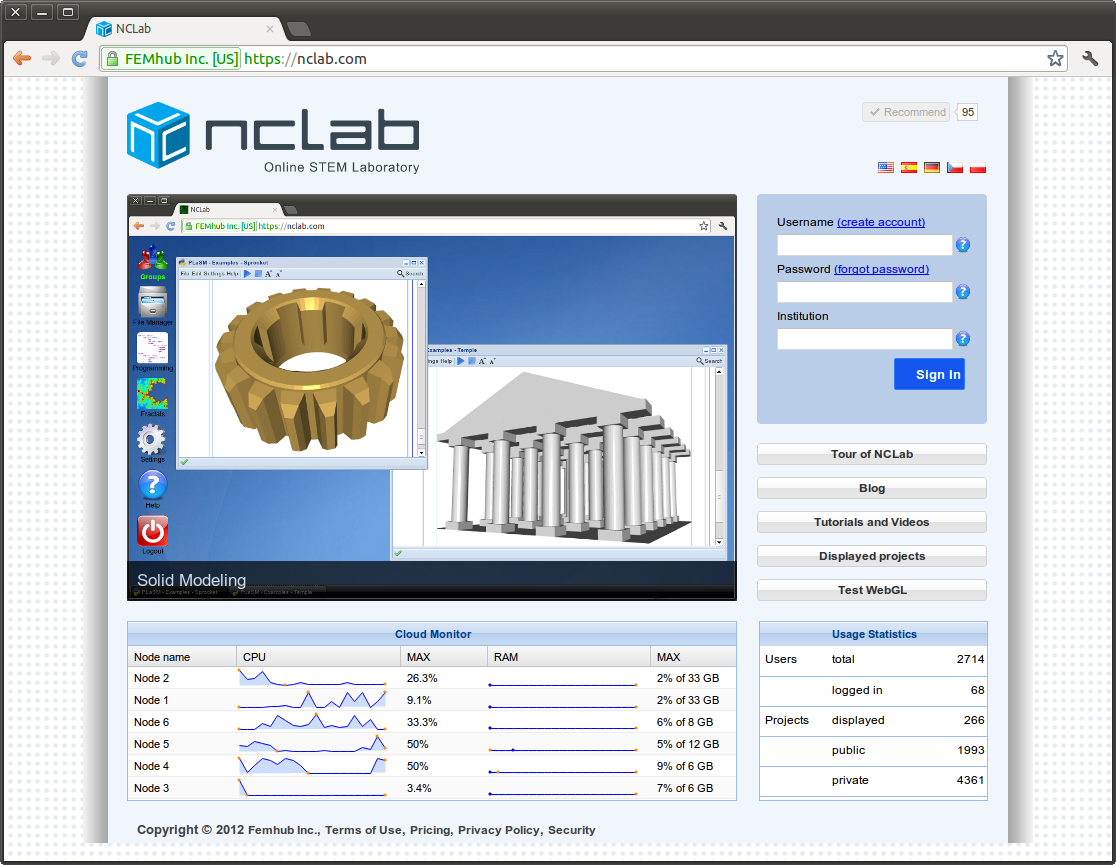
\includegraphics[width=\textwidth]{img/outside.png}
\end{center}
\vspace{-2mm}
\caption{NCLab's home page.}
\label{fig:outside}
%\vspace{-0.6cm}
\end{figure}

\noindent
The User Statistics window, located in the 
bottom-right corner, provides current overview of NCLab's users and their projects. 
The window above User Statistics is a WebGL tester. WebGL is a very recent 
web-browser technology that supports {\em amazing} 3D graphics. 

\subsection{WebGL}

WebGL is a web browser analogy of OpenGL (realistic hardware-supported 3D graphics). 
The technology is so new that it is 
turned off in some web browsers by default. It should work in modern web browsers 
(not Internet Explorer) and on reasonable new computers. To test whether your web 
browser and graphic card support it,  
click on the "Test WebGL" button. If you see a window 
similar to the one in Fig. \ref{fig:webgl2} then you are fine. 

\begin{figure}[!ht]
\begin{center}
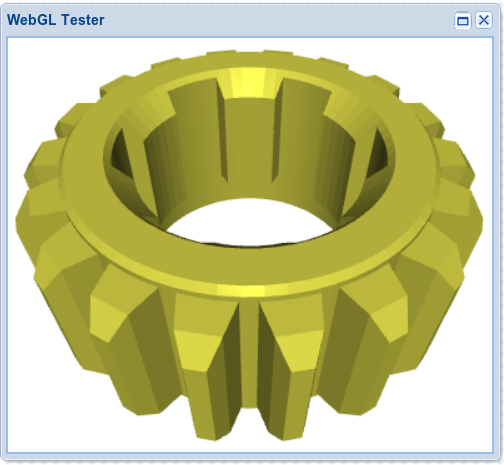
\includegraphics[width=0.5\textwidth]{img/webgl2.png}
\end{center}
\vspace{-2mm}
\caption{WebGL Tester.}
\label{fig:webgl2}
\end{figure}
\noindent
Now you can click into the WebGL tester window, and move 
your mouse while keeping the left button pressed, to see WebGL in action.

However, you may also see a message similar to the one shown in Fig. \ref{fig:nowebgl}.
\newpage
\begin{figure}[!ht]
\begin{center}
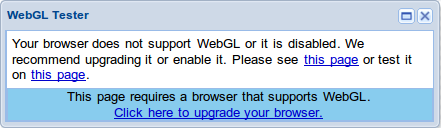
\includegraphics[width=0.7\textwidth]{img/nowebgl.png}
\end{center}
\vspace{-2mm}
\caption{Message saying that WebGL is not enabled.}
\label{fig:nowebgl}
\end{figure}
\noindent
There may be multiple reasons for this message:
\begin{enumerate}
\item {\em You are using Internet Explorer (IE)}. IE does not have WebGL support. If you are using this web browser, please install another 
one such as Chrome, Firefox, Safari etc. This takes only minutes (at most) and it is highly rewarding in terms 
of improved Internet experience. In fact, poor performance of IE was causing such problems to NCLab users that 
we eventually decided to banish IE. 
\item {\em Your browser is outdated.} We recommend that you upgrade your web browser to the newest version, this 
can never hurt. 
\item {\em Your browser has WebGL disabled.} Try to get into the Settings of your browser (in Firefox this is via 
{\tt about:flags}) and search for "WebGL". Once you find it, enable it. You will be asked to restart your web browser.
\item {\em Everything failed.} In this case, try to upgrade your graphics drivers. This should help. If you still have 
problems, go to the page {\tt www.webgl.org} and try to find help there. You can also google for "graphic cards that 
support webgl" which will give you and idea whether your graphic card s supported or not. 
\item As a general observation, WebGL works almost always in Safari on more recent Mac systems  
\end{enumerate}

\subsection{Creating an Account}

A login dialog where
users enter their username, password and institution code is located in the 
top-right corner. In order to create a new account, click on the link "Create free account" which is next to
"Username". The following window appears:

\newpage

\begin{figure}[!ht]
\begin{center}
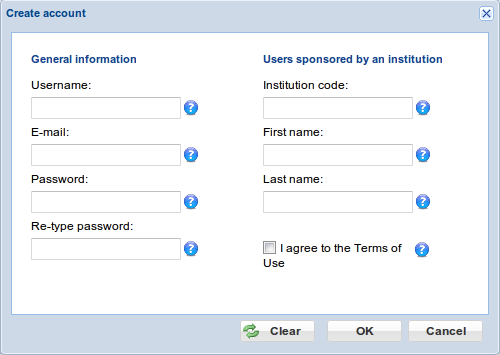
\includegraphics[width=0.7\textwidth]{img/create-account.png}
\end{center}
\vspace{-4mm}
\caption{Creating new account.}
\label{fig:creacc}
\end{figure}

\noindent
In this form, enter your preferred username, email address (to be used only if you ask
us to generate a new password for you), and password twice. Next:

\begin{itemize}
\item If you belong to an institution 
      that uses NCLab for teaching or research, you should know your institution's code. Enter it in the form, 
      along with your first and last names. Your name will be visible to an NCLab admin
      who will verify that you belong to the institution.
\item If you are using NCLab for your personal hobby or self-education, for activities not 
      related to any institutional use, then leave the last three lines empty. 
\end{itemize}
After accepting the Terms of Use and clicking OK, you are ready to login!

\subsection{After Login}

The interior of NCLab is similar to a standard computer desktop, except that the 
icons are different (Fig. \ref{fig:desktop}). Many users maximize 
the web browser window to make the desktop experience even more realistic.
If any member of any of your groups is in NCLab at the time you log in, the Groups icon 
will be lighted green.

\newpage

\begin{figure}[!ht]
\begin{center}
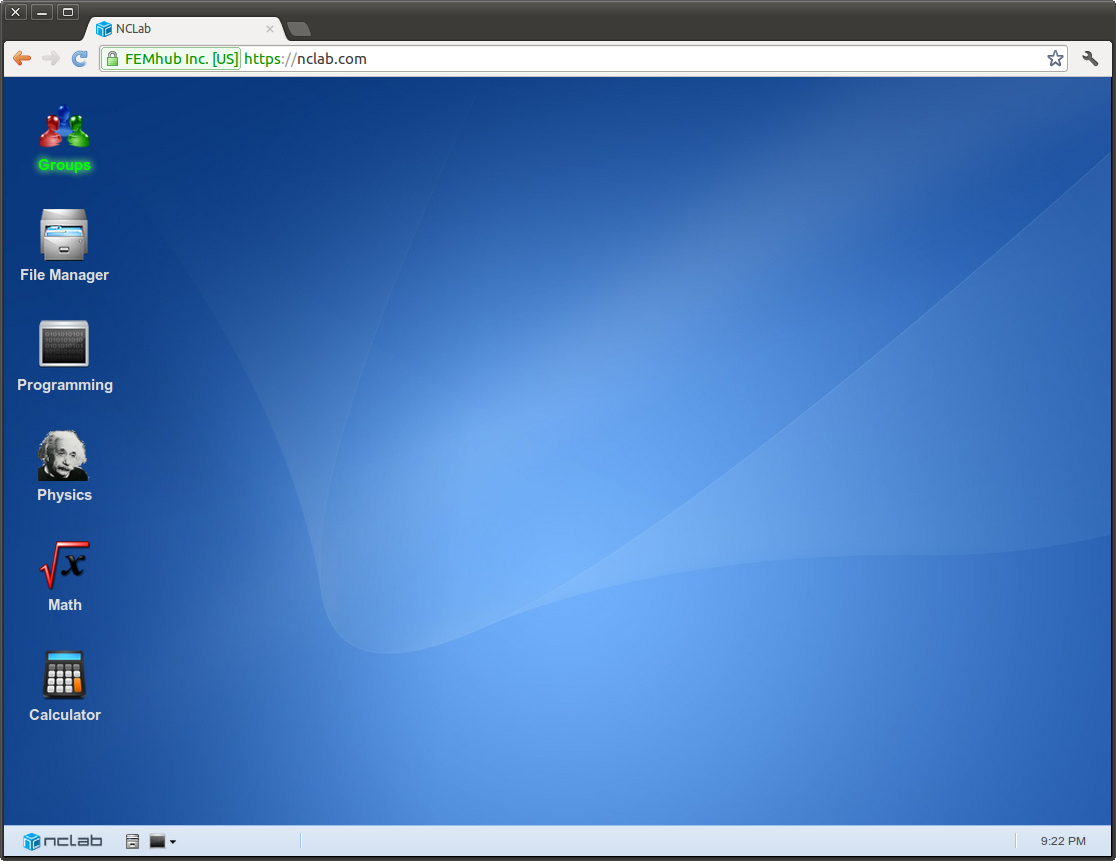
\includegraphics[width=\textwidth]{img/desktop.png}
\end{center}
%\vspace{-2mm}
\caption{NCLab desktop after login. The green light at "Groups" means that someone in your 
         groups is online.}
\label{fig:desktop}
\end{figure}
\noindent
If you do not like the default desktop background, it can be changed easily in Settings, as shown in 
Fig. \ref{fig:desktop}.
\newpage
\begin{figure}[!ht]
\begin{center}
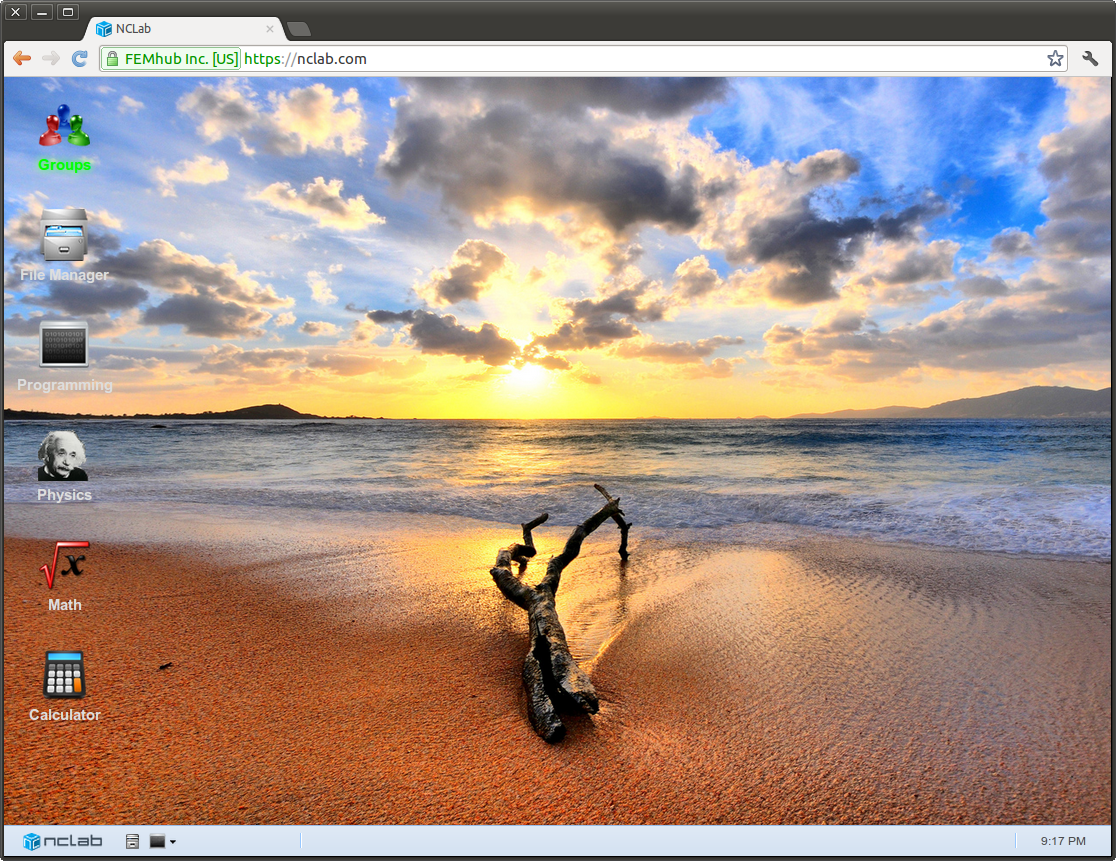
\includegraphics[width=\textwidth]{img/desktop2.png}
\end{center}
%\vspace{-2mm}
\caption{Changing desktop background.}
\label{fig:desktop2}
\end{figure}
\noindent


\noindent
Groups were already mentioned. The other icons
represent:

\begin{itemize}
\item {\em File Manager}, used to manage files and folders, and to clone work published by other users.
\item {\em Programming} module provides programming in 
      \begin{itemize}
      \item Karel the Robot (popular educational language for beginners).
      \item Python (modern programming language for advanced applications). Python is 
            very popular in engineering and science because it is interpreted (not compiled as C or C++),
            has simple syntax, and comes with powerful libraries.
      \item Javascript (most popular language for web development). 
      \item CUDA (massively parallel programming on graphic cards).
      \item Web Design with HTML, Javascript (JS) and CSS. 
      \end{itemize}
\item {\em Physics} module provides various physics simulation tools in Kinematics,
      Solid Mechanics, Fluid Dynamics, Electromagnetics, and other areas. 
\item {\em Math} module offers Fractal Explorer (interactive graphical application 
      to explore Fractals and generate beautiful fractal art), ODE module to explore 
      ordinary differential equations, and PDE module to explore partial differential 
      equations. 
\item {\em Calculator} is a calculator! 
\end{itemize}
More modules are on the way. 

\subsection{Groups and Chat}

In NCLab, users can form groups, see who is online, and chat in real time. In order to 
create a new group, click on the Groups icon. A window similar to the one shown 
in Fig. \ref{fig:groups} appears. This concrete screenshot shows four groups of the 
user "solin" -- the top one was created by Jordan, the other three by solin. The 
green light next to the last group indicates that someone in that group
is currently in NCLab. Before we go look who that is, note that you can create a
new group of your own by clicking on "New Group". In order to add people to your groups,
you need to know their usernames. The button "Who's online" allows you to see instantly 
all users in all your groups who are currently logged in. 

\begin{figure}[!ht]
\begin{center}
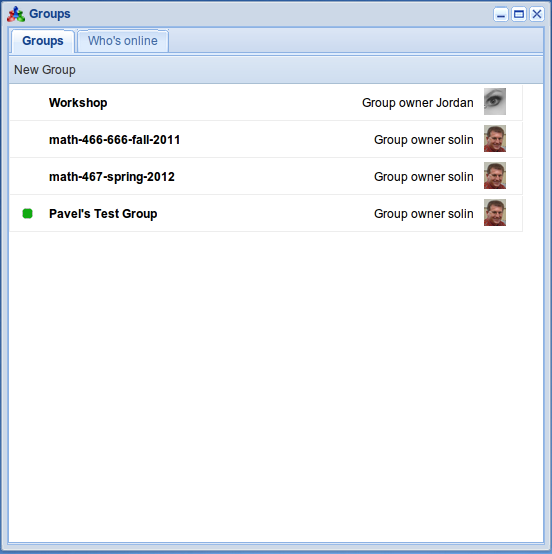
\includegraphics[width=0.5\textwidth]{img/groups.png}
\end{center}
%\vspace{-2mm}
\caption{Groups window, showing that someone in the last group is currently in NCLab.}
\label{fig:groups}
\end{figure}

\newpage
\noindent
Clicking on the last group 
reveals that the online users are Emily and Rick.
\begin{figure}[!ht]
\begin{center}
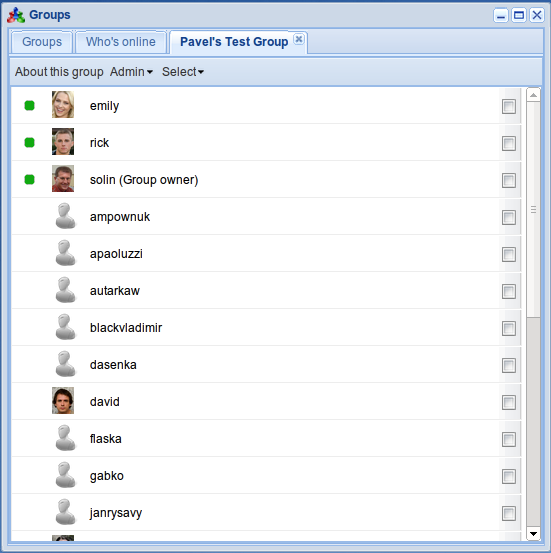
\includegraphics[width=0.5\textwidth]{img/groups-2.png}
\end{center}
%\vspace{-2mm}
\caption{Detail of the last group.}
\label{fig:groups-2}
\end{figure}

\noindent
Clicking on any user who has the green light next to him/her (except yourself),
you initiate a chat to that user. Or someone from your groups may contact you. 
The Chat window is shown in Fig. \ref{fig:chat}.

\begin{figure}[!ht]
\begin{center}
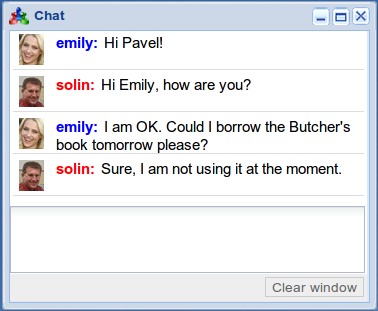
\includegraphics[width=0.4\textwidth]{img/chat.png}
\end{center}
%\vspace{-2mm}
\caption{Chat window.}
\label{fig:chat}
\end{figure}

\subsection{File Manager}

Clicking on the File Manager icon launches the application. Initially, you will not 
have any files or folders there (Fig. \ref{fig:fileman}).

\begin{figure}[!ht]
\begin{center}
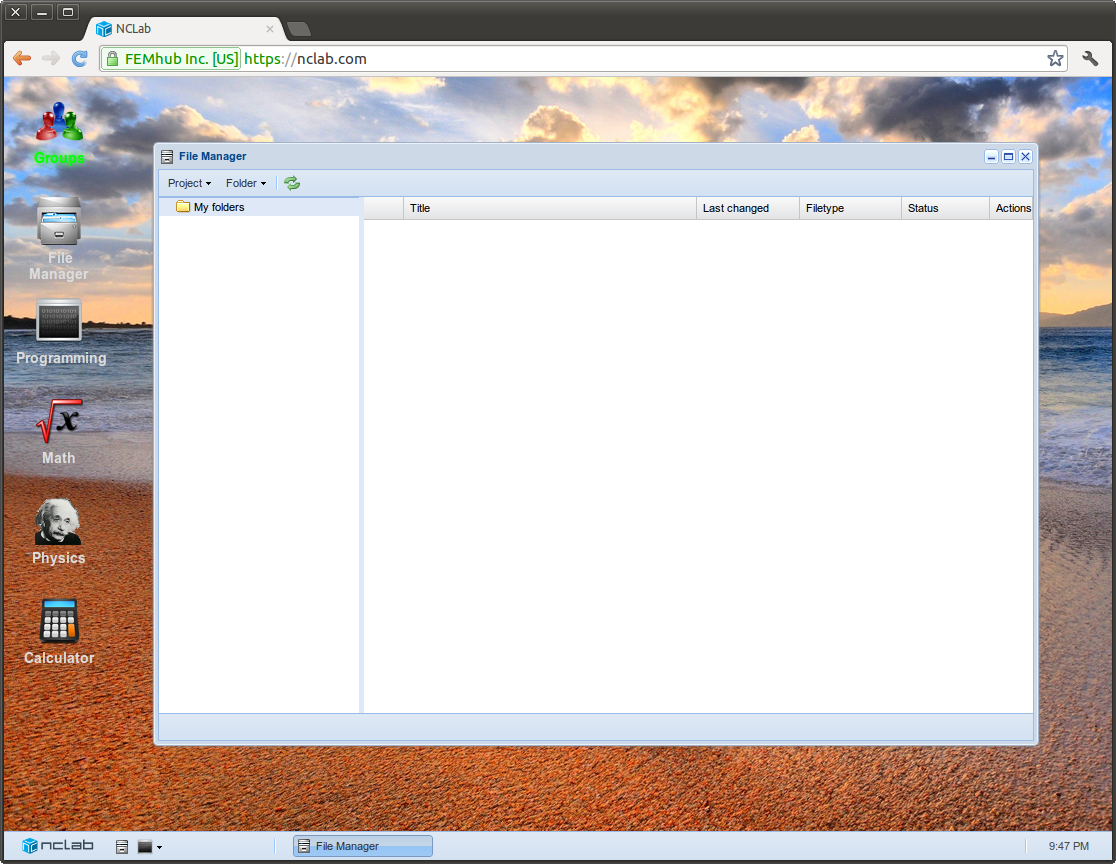
\includegraphics[width=\textwidth]{img/fileman1.png}
\end{center}
%\vspace{-2mm}
\caption{Initial launch of File Manager.}
\label{fig:fileman}
\end{figure}
\noindent
However, this can be changed quickly. Click on the menu Project $\rightarrow$ Clone. This will
launch a window with many displayed projects from various areas of programming, web design, math, 
physics, 3D computer aided design, and engineering simulations (Fig. \ref{fig:fileman2}).

\newpage

\begin{figure}[!ht]
\begin{center}
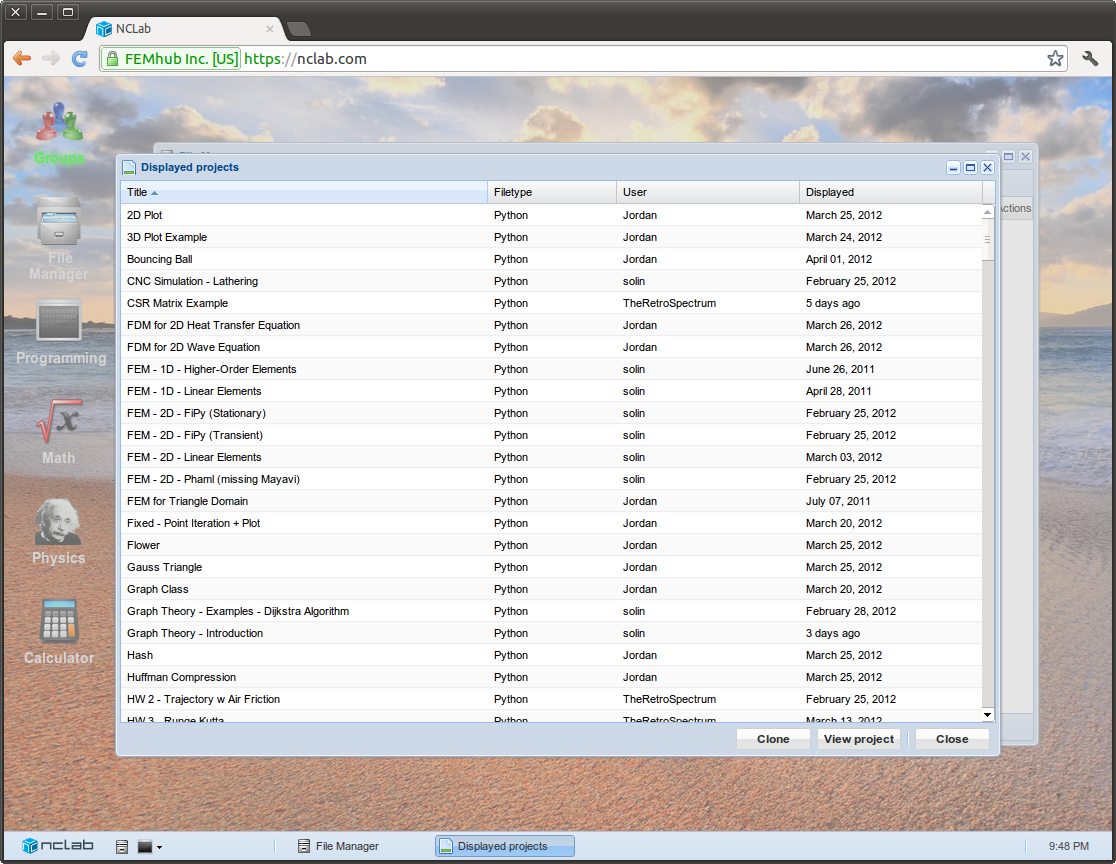
\includegraphics[width=\textwidth]{img/fileman2.png}
\end{center}
%\vspace{-2mm}
\caption{List of displayed projects.}
\label{fig:fileman2}
\end{figure}
\noindent
You can view the contents of any displayed project by double-clicking on it. You can 
clone any project into your account by just clicking on it once, and then clicking on 
the button "Clone". Let's say that we want to learn Python programming. After cloning 
the project "Python - Intro", we will see the following in the File Manager:

\newpage

\begin{figure}[!ht]
\begin{center}
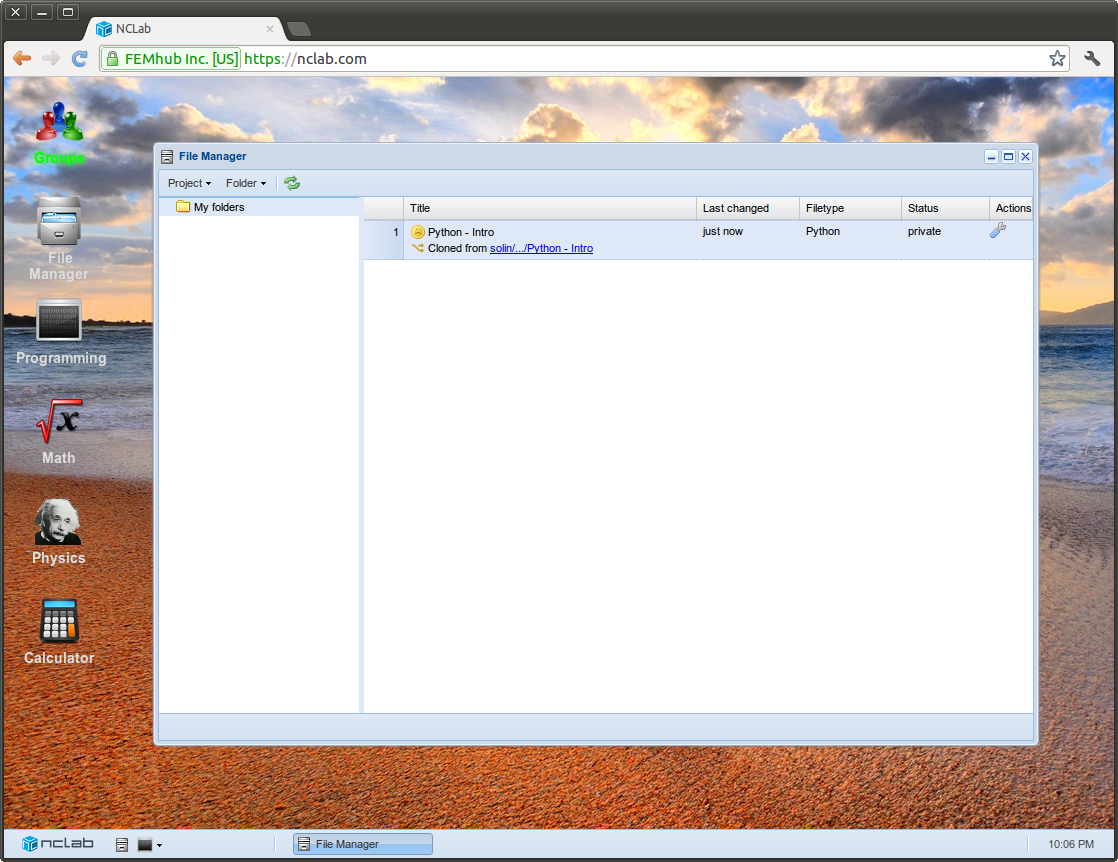
\includegraphics[width=\textwidth]{img/fileman3.png}
\end{center}
%\vspace{-2mm}
\caption{After cloning the project "Python - Intro".}
\label{fig:fileman3}
\end{figure}
\noindent
Now by clicking on the project, it launches in a new window, as
shown in Fig. \ref{fig:fileman4}.

\newpage

\begin{figure}[!ht]
\begin{center}
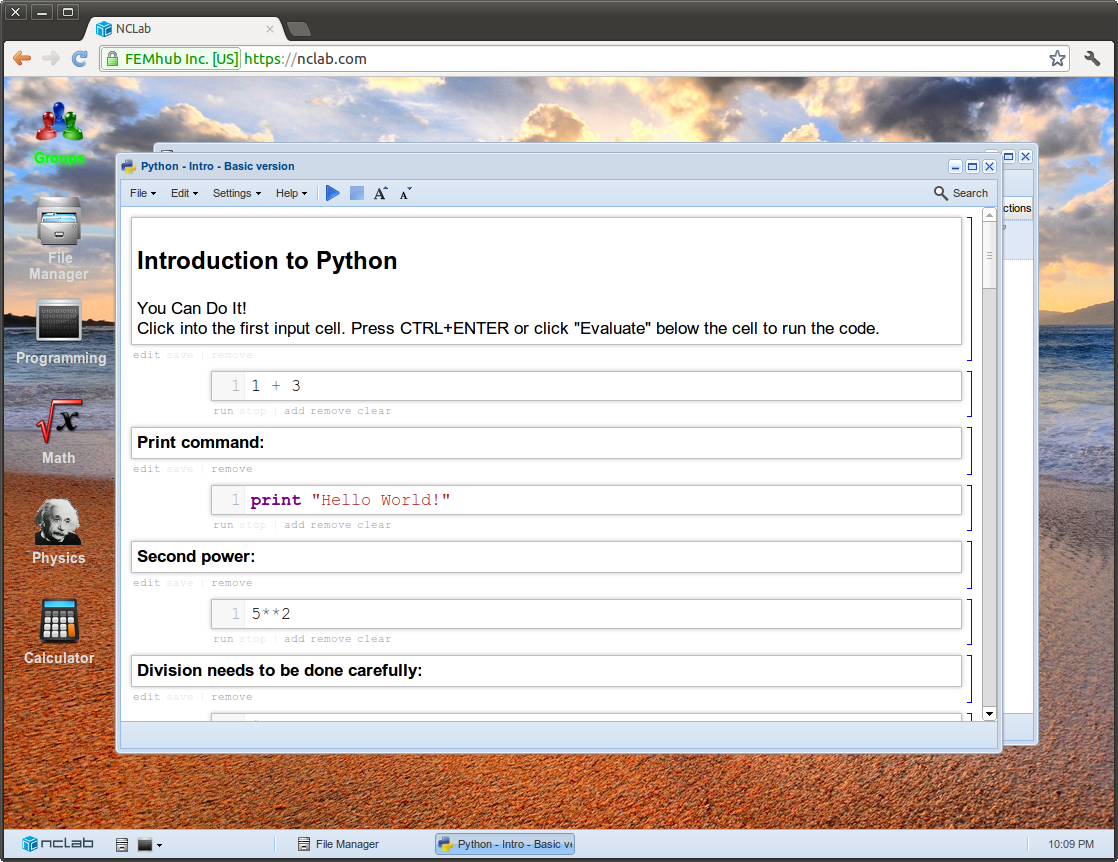
\includegraphics[width=\textwidth]{img/fileman4.png}
\end{center}
%\vspace{-2mm}
\caption{Launching project "Python - Intro".}
\label{fig:fileman4}
\end{figure}
\noindent
The worksheet contains {\em input cells} where you can enter or edit computer
code, and descriptive {\em text cells}. The contents of text cells can be 
edited after clicking on the cell. The text is be formatted using Restructured
Text (RST) format. You can click on the blue arrow button to evaluate all input 
cells in the worksheet (hold on with that for a moment), or you can evaluate 
each input cell individually by clicking on the "run" right under it. 

Let us evaluate the first input cell that contains just {\tt 1 + 3}. This will send its contents 
to the server where it will be parsed using a Python interpreter, and the 
output will be sent back to your browser and displayed almost instantly in
a new yellow {\em output cell} (Fig. \ref{fig:fileman5}).

\newpage

\begin{figure}[!ht]
\begin{center}
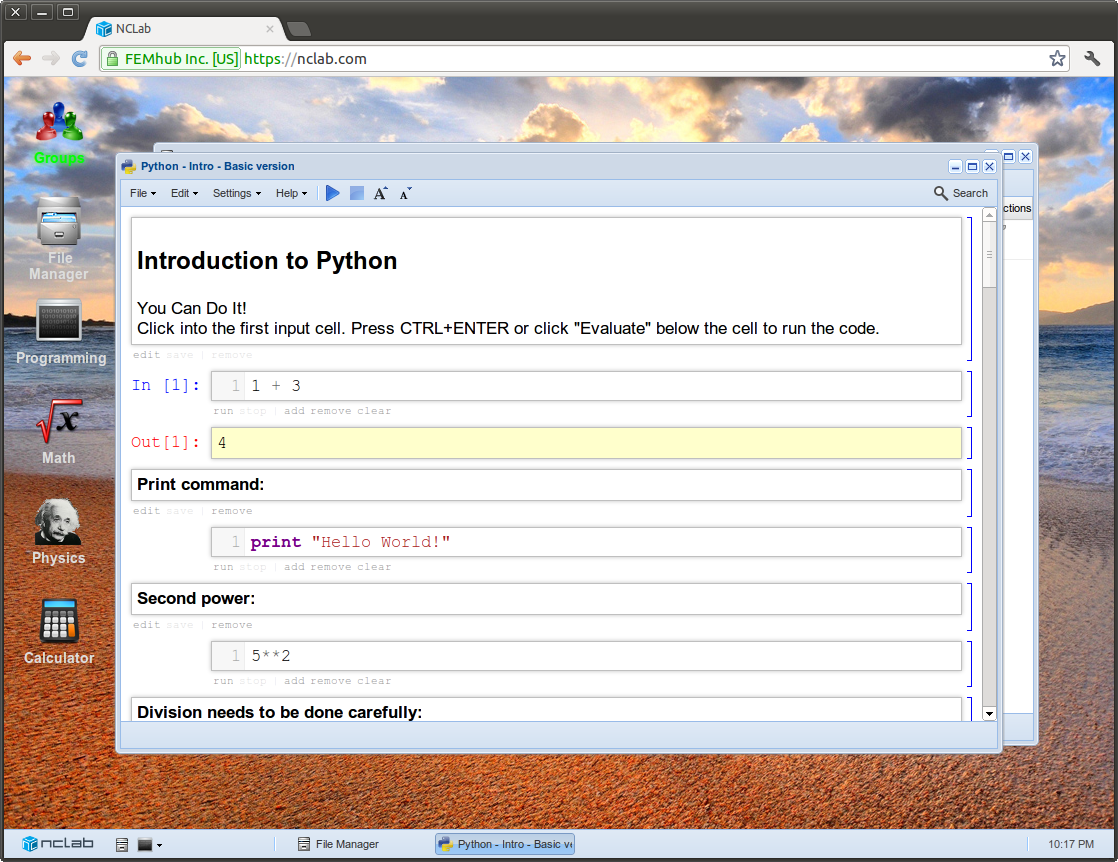
\includegraphics[width=\textwidth]{img/fileman5.png}
\end{center}
%\vspace{-2mm}
\caption{Output is displayed in yellow {\em output cells}.}
\label{fig:fileman5}
\end{figure}
\noindent
We recommend that you spend some time experimenting with the 
File Manager's menu and this worksheet. Try to:
\begin{itemize}
\item Insert new input cells below and about an existing input cell.
\item Insert new text cells below and about an existing input cell.
\item Remove cells by clicking on "remove" under tehm.
\item Create a new folder "Python" and drag your cloned Python 
      project in there. 
\item Rename the file and folder.
\item Duplicate your project via "Save as" under a different name.
\item Synchronize your cloned project with the original via the 
      "Synchronize" button. Beware though - synchronizing discards 
      all your changes that you made to the project since cloning. 
\item Access a Python Tutorial via the Help button.
\end{itemize}

\section{Programming Module}

Clicking on the Programming icon launches programming menu that 
contains several languages and a web design application:

\begin{figure}[!ht]
\begin{center}
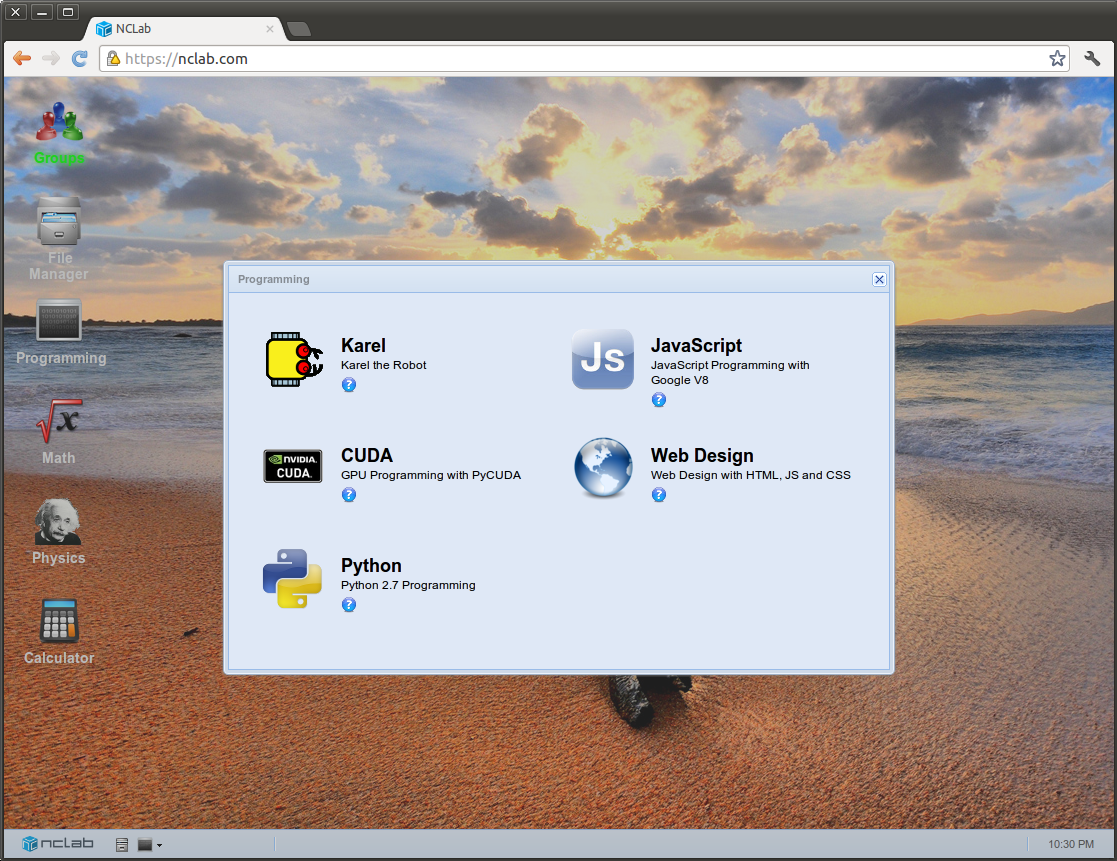
\includegraphics[width=\textwidth]{img/progr1.png}
\end{center}
%\vspace{-2mm}
\caption{Programming menu.}
\label{fig:progr1}
\end{figure}
\noindent
Each programming language here comes with a Help of its own, so we 
will be brief. 

\subsection{Karel the Robot}

Clicking on "Karel" launches the famous educational 
programming language Karel the Robot that was created at the Stanford 
University and is used to teach programming in many countries all over 
the world (Fig. \ref{fig:progr2}). Teachers prefer Karel over other 
educational languages because of its minimum overhead (students can 
start programming in the first class) and because a smooth transition 
to Python.

\begin{figure}[!ht]
\begin{center}
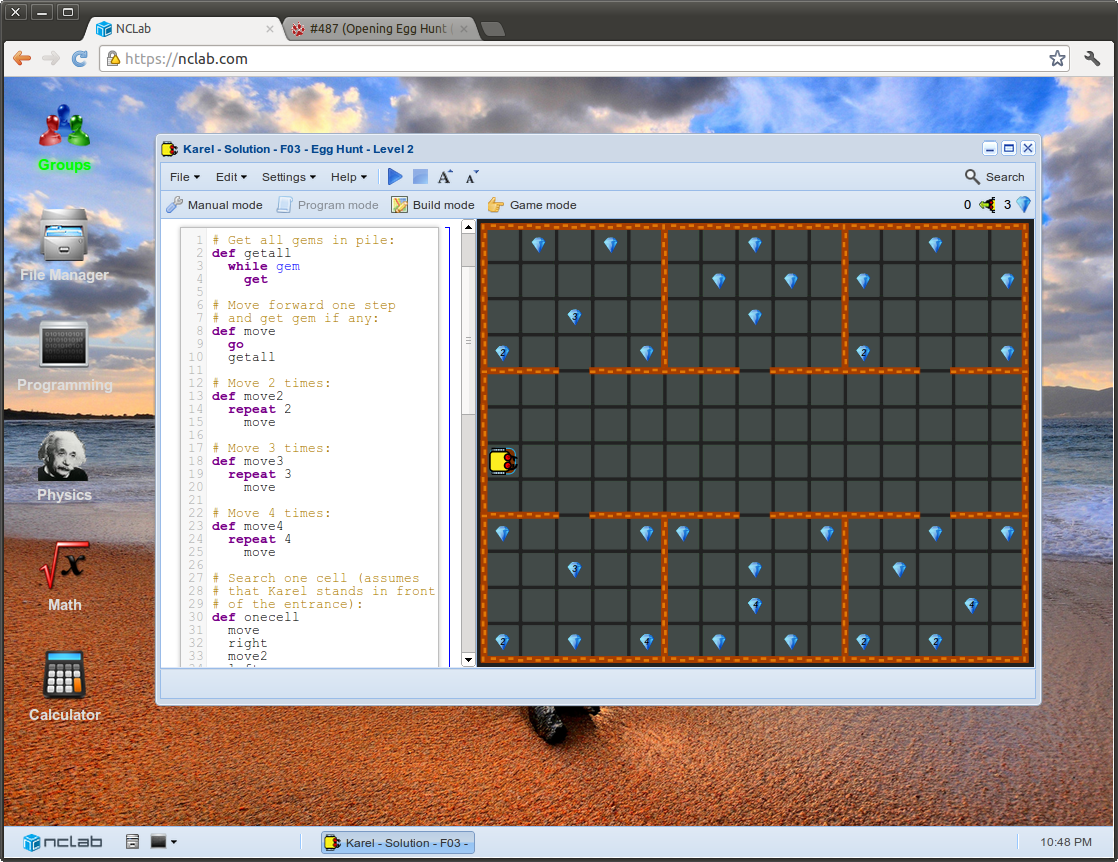
\includegraphics[width=\textwidth]{img/progr2.png}
\end{center}
%\vspace{-2mm}
\caption{Karel the Robot - illustrative screenshot.}
\label{fig:progr2}
\end{figure}
\noindent
Textbook, Solution Manual and a YouTube Video are available via the link "Tutorials and Videos"
on NCLab's front page. There is an extensive suite of exercises (games) among 
displayed projects that you can clone into your account. All of them are described in the 
tutorial.

\subsection{Python}

Clicking on the Python icon in the Programming Module launches Python 
worksheet, where you can start programming instantly (Fig. \ref{fig:progr3}).
 
\begin{figure}[!ht]
\begin{center}
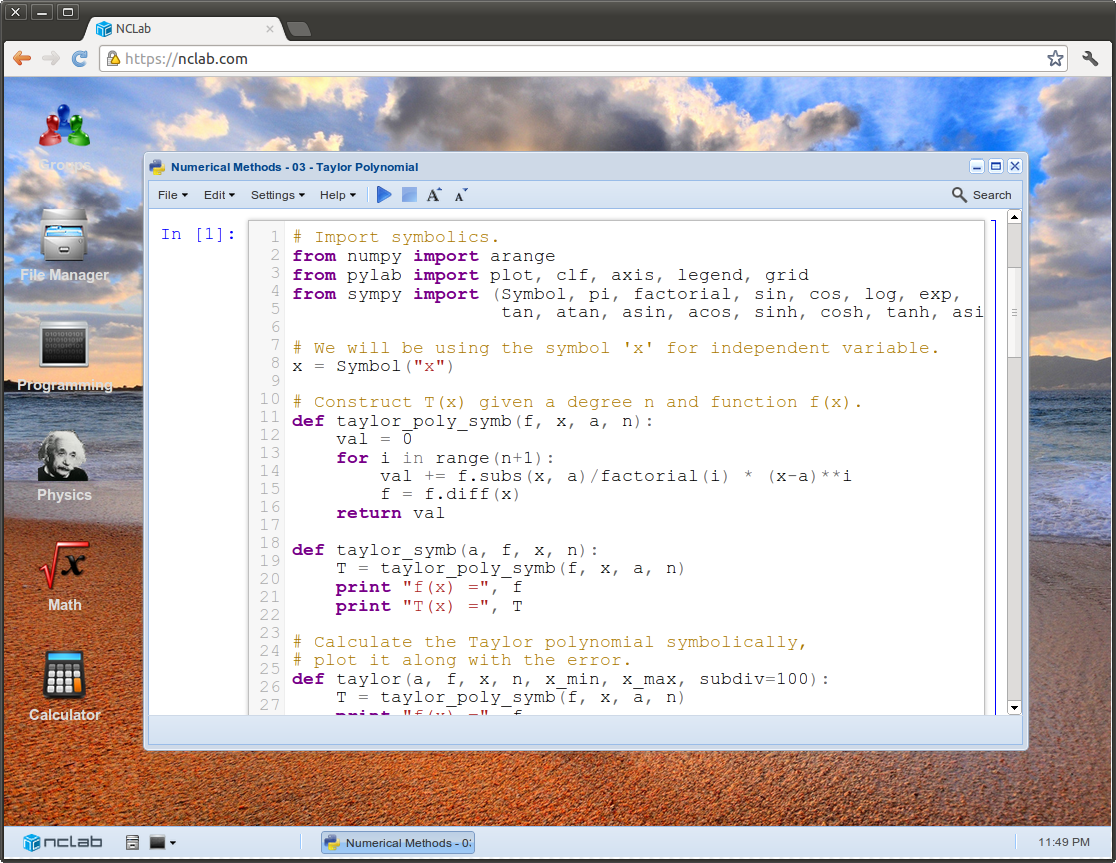
\includegraphics[width=\textwidth]{img/progr3.png}
\end{center}
%\vspace{-2mm}
\caption{Python programming - illustrative screenshot.}
\label{fig:progr3}
\end{figure}
\noindent
The interpreter on the server side is Python 2.7 and Python 3.3 is in preparation. 
Textbook is available via the link "Tutorials and Videos" on NCLab's front page
and via the Help button. 

\subsection{Parallel computing with GPUs}

GPU stands for {\em Graphics Processing Unit} and massively parallel computing with GPUs
is one of the hottest new trends in Computational Science. The main advantage 
of GPUs over standard CPUs (Central Processing Units) is that on the same price 
level, GPUs provide much larger number of cores and Flops (number of floating 
operations per second) compared to CPUs.
 
CUDA is an Nvidia language for GPUs. The CUDA worksheet provides programming via 
PyCUDA (Python wrappers to CUDA). Tutorial to PyCUDA is available via the link "Tutorials and Videos" 
on NCLab's front page and via the Help button, and there are around 30 
displayed projects where you can learn both basic and advanced aspects of CUDA
programming. 

\begin{figure}[!ht]
\begin{center}
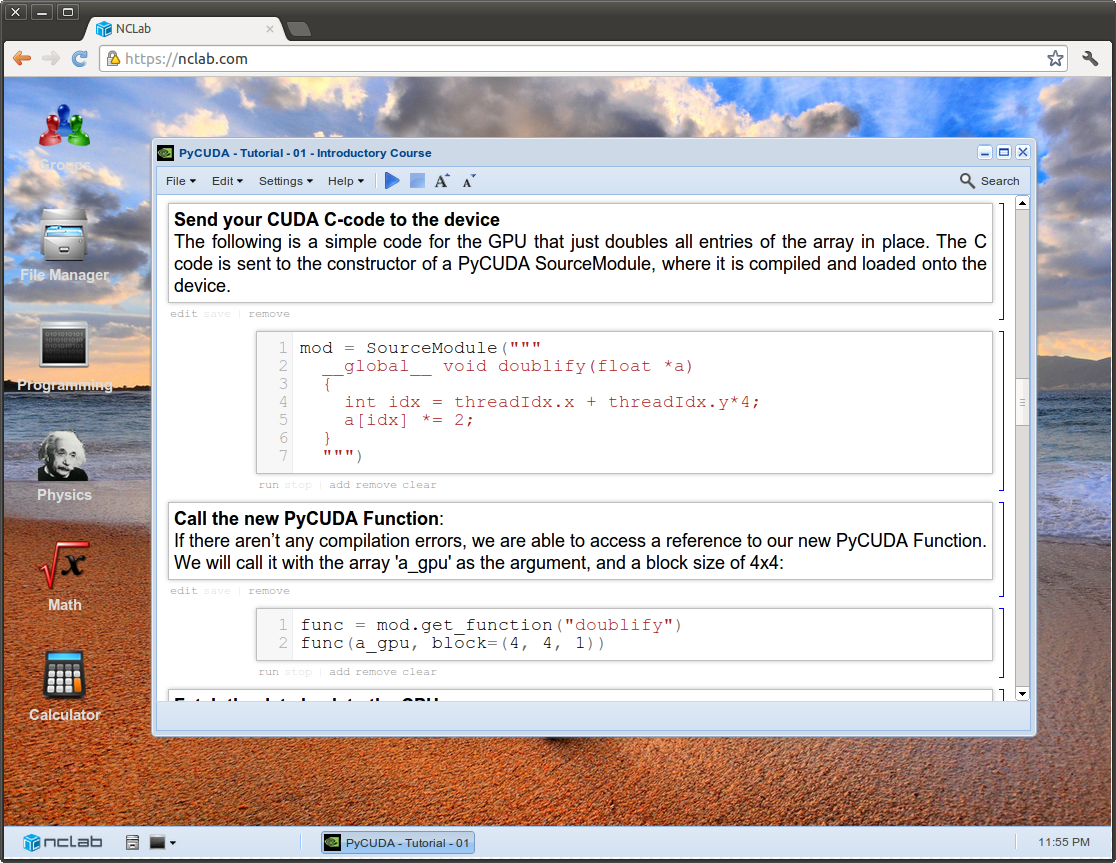
\includegraphics[width=\textwidth]{img/progr4.png}
\end{center}
%\vspace{-2mm}
\caption{CUDA programming - illustrative screenshot.}
\label{fig:progr4}
\end{figure}
\noindent


\subsection{Javascript}

The Javascript (JS) worksheet provides JS programming using the Google V8 engine 
on server side. In other words, the Javascript is not processed in the web browser but 
on the remote server similarly to Python. 
\newpage
\begin{figure}[!ht]
\begin{center}
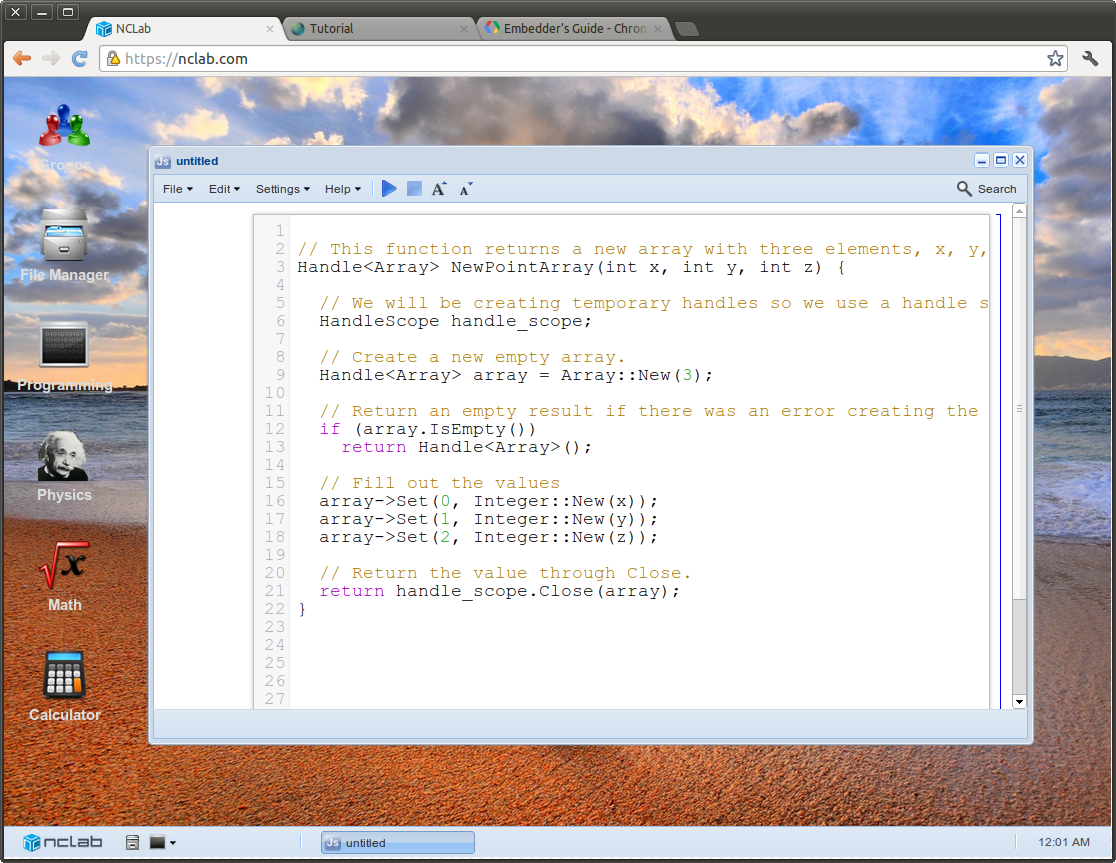
\includegraphics[width=\textwidth]{img/progr5.png}
\end{center}
%\vspace{-2mm}
\caption{Javascript programming based on Google V8 - illustrative screenshot.}
\label{fig:progr5}
\end{figure}
\noindent
More information is available in the Help section.

\subsection{WebDesign}

The Web Design kit is an integrated environment for the design of web pages.
The graphical application contains three input panels for HTML, JS and CSS, and 
one output panel. The web page is changing in real time when any of the three 
input panels are edited. The output panel can be detached and magnified for better 
viewing comfort. Users belonging to an institutions and 
users operating NCLab in Full Version can have their web pages hosted.

\begin{figure}[!ht]
\begin{center}
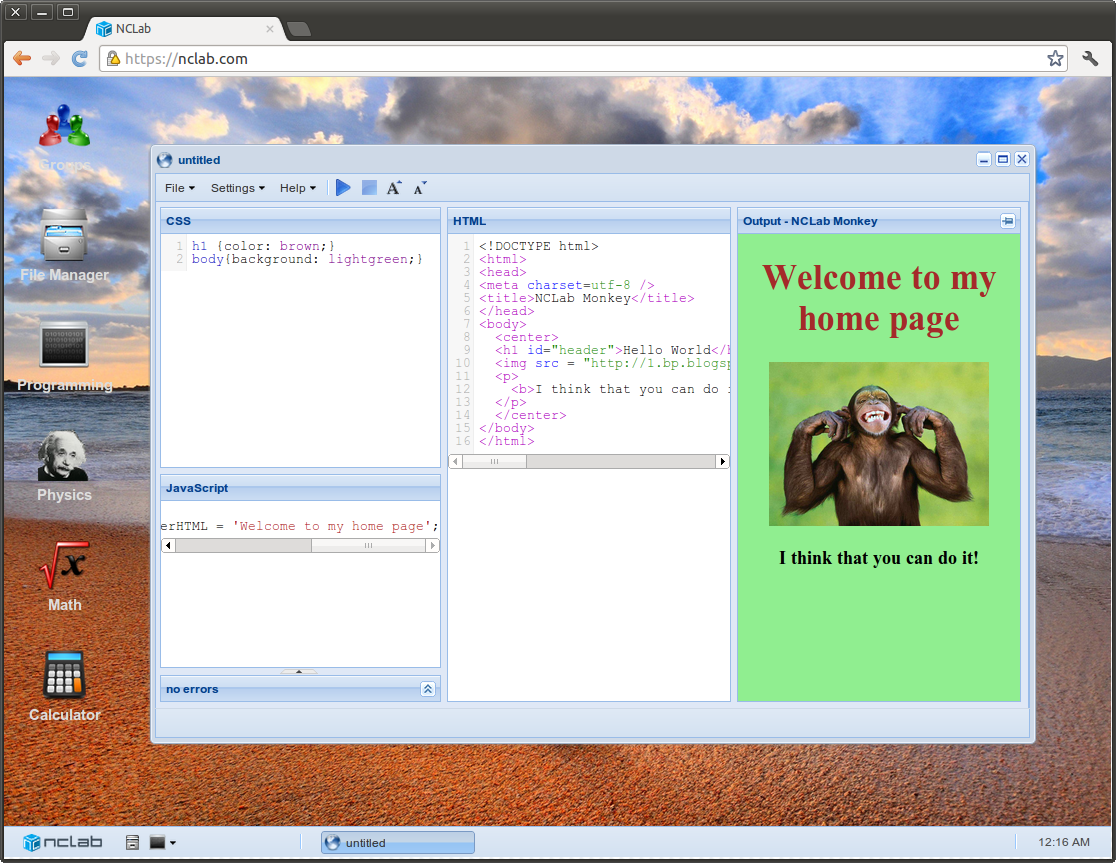
\includegraphics[width=\textwidth]{img/progr6.png}
\end{center}
%\vspace{-2mm}
\caption{Web Design kit - illustrative screenshot.}
\label{fig:progr6}
\end{figure}
\noindent
More information is available in the Help section.

\section{Physics Module}

The Physics module contains a quickly growing number of graphical applications 
from many different areas including kinematics, solid mechanics, 
fluid dynamics, electromagnetics, and others.

\subsection{Kinematics}

Kinematics deals with moving objects.  
Classical application from this field -- Projectile Motion -- enables computing 
the trajectory of a flying projectile either with or without considering 
air friction. Illustrative screenshot is shown in Fig. 
\ref{fig:kinem1}. 
\newpage
\begin{figure}[!ht]
\begin{center}
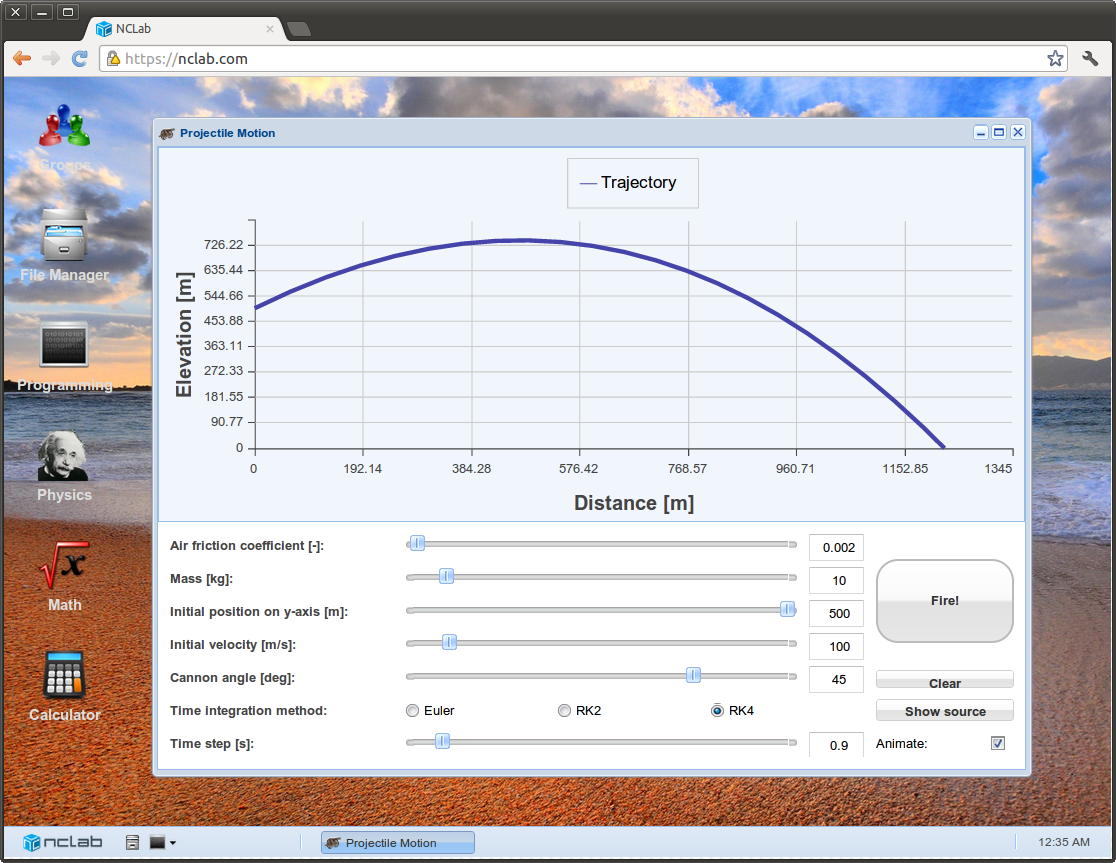
\includegraphics[width=\textwidth]{img/kinem1.png}
\end{center}
%\vspace{-2mm}
\caption{Projectile motion.}
\label{fig:kinem1}
\end{figure}
\noindent

\subsection{Solid Mechanics}

Solid mechanics deals with deformation of solid objects. NCLab 
offers an Elasticity module that allows the user to define an
arbitrary 2D object, define its material properties (density, Young modulus, 
Poisson ratio), prescribe displacements and acting forces on the boundary, 
and calculate displacements and stresses inside the object. This application  
uses the Hermes library (http://hpfem.org/hermes) for the finite element 
analysis (FEA) part. Illustrative screenshot is provided in Fig. \ref{fig:elast1}.
\newpage
\begin{figure}[!ht]
\begin{center}
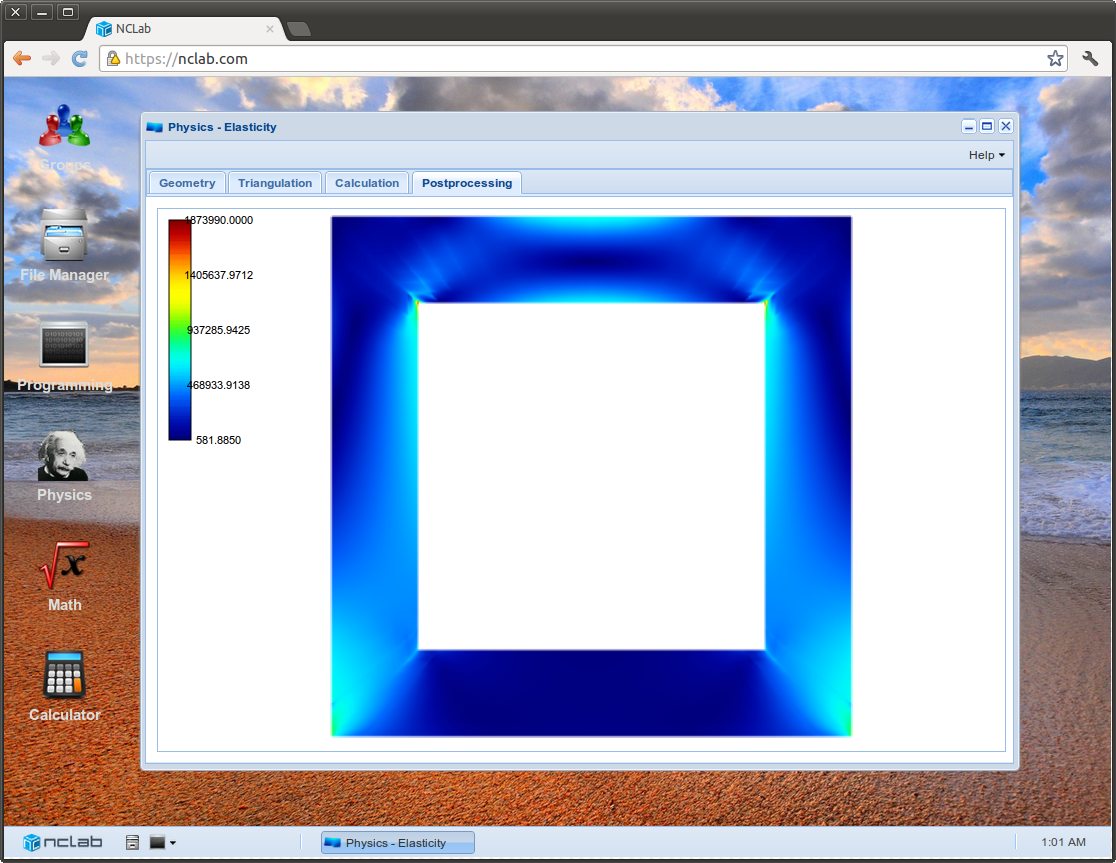
\includegraphics[width=\textwidth]{img/elast1.png}
\end{center}
%\vspace{-2mm}
\caption{Elasticity analysis of a hollow steel pipe of square cross-section that is loaded from above.}
\label{fig:elast1}
\end{figure}
\noindent
The simulation process consists of several steps: geometry definition, 
mesh generation, problem definition, computaion, and postprocessing. 
The application will walk you through these steps, and Help 
is available for each of them.

\subsection{Electromagnetics}

The Electromagnetics module contains at the moment two modules: an axisymmetric 
capacitor model and a general electrostatics model. In both cases one calculates 
the distribution of the electric field surrounding charged objects. Boundary 
conditions can be prescribed voltage on some part of the boundary and / or 
prescribed electric charge density on another part of boundary. Two illustrative 
screenshots of the capacitor model are provided below.
\newpage
\begin{figure}[!ht]
\begin{center}
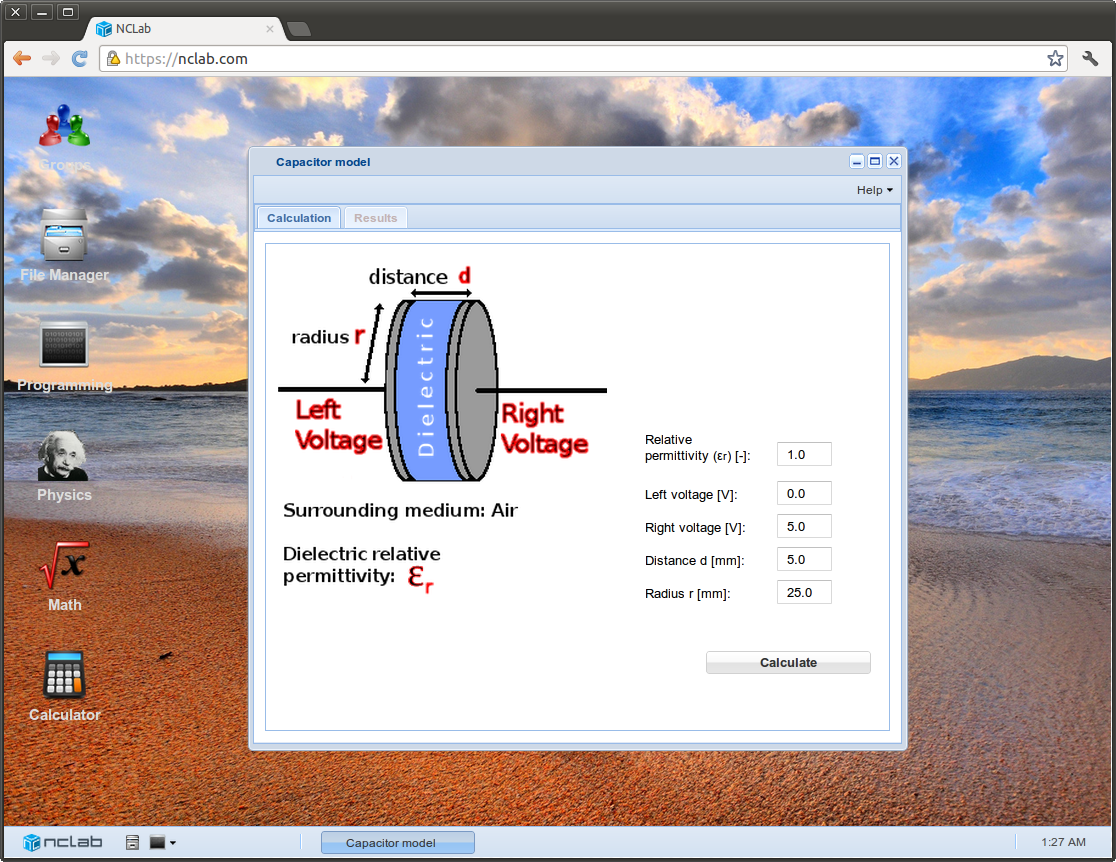
\includegraphics[width=\textwidth]{img/capac1.png}
\end{center}
%\vspace{-2mm}
\caption{Plate capacitor - axisymmetric model.}
\label{fig:capac1}
\end{figure}
\noindent

\newpage

\begin{figure}[!ht]
\begin{center}
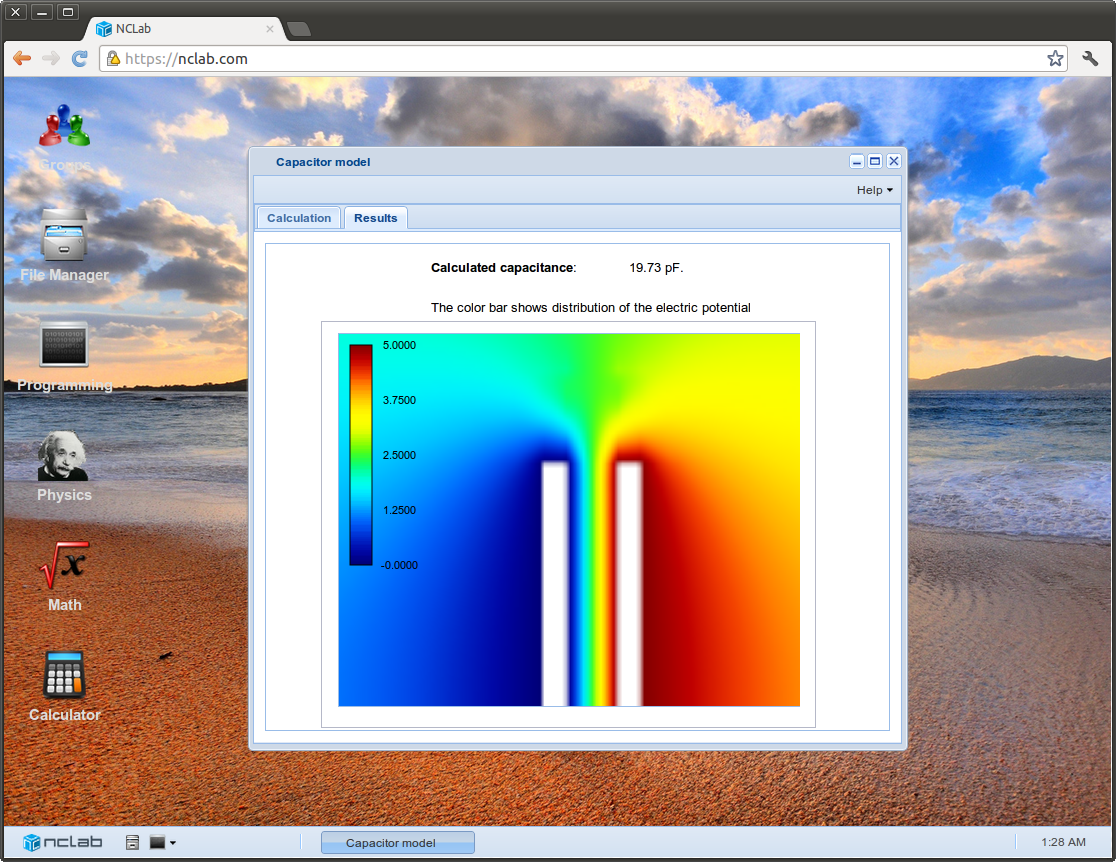
\includegraphics[width=\textwidth]{img/capac2.png}
\end{center}
%\vspace{-2mm}
\caption{Capacitor model - results.}
\label{fig:capac2}
\end{figure}
\noindent


\subsection{Fluid Dynamics}

The Fluid Dynamics module contains a model of draining a tank filled with water. 
Illustrative screenshot is shown in Fig. \ref{fig:tank1}.

\newpage

\begin{figure}[!ht]
\begin{center}
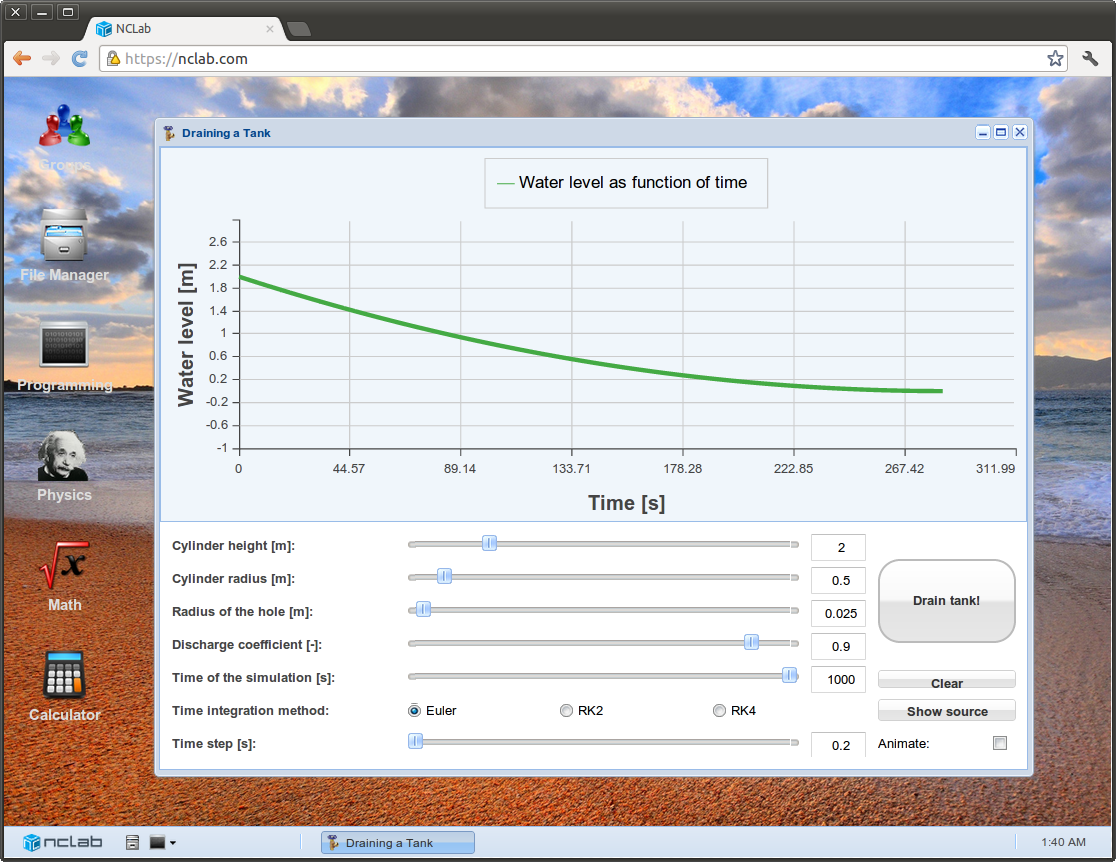
\includegraphics[width=\textwidth]{img/tank1.png}
\end{center}
%\vspace{-2mm}
\caption{Draining a tank with water.}
\label{fig:tank1}
\end{figure}



\section{Math Module}

The Math module contains several graphical applications including the Fractal 
Explorer, and applications for ordinary differential equations (ODE) and partial 
differential equations (PDE). Besides this, symbolic and numerical math 
as well as graph theory are available through Python libraries Sympy,
Numpy, Scipy, Pylab, NetworkX and others. These will be discussed in the following 
documents.

\subsection{Fractal Explorer}

The Fractal Explorer allows you to get acquainted with beautiful 
fractal structures of the Mandelbrot and Julia sets. Tutorial 
is available via the "Tutorials and Videos" link on NCLab's front page. 
Sample screenshot showing a Julia set is below:

\begin{figure}[!ht]
\begin{center}

\includegraphics[width=0.7\textwidth]{img/julia.png}
\end{center}
%\vspace{-2mm}
\caption{Julia fractal.}
\label{fig:julia}
\end{figure}




\subsection{ODE}

Part of the Ordinary Differential Equations (ODE) section are advanced Java applets JODE by Marek 
Rychlik (University of Tucson) for plotting slope fields and solutions 
of two-ODE and three-ODE systems. Illustrative screenshot of the slope 
field application is below.

\newpage

\begin{figure}[!ht]
\begin{center}
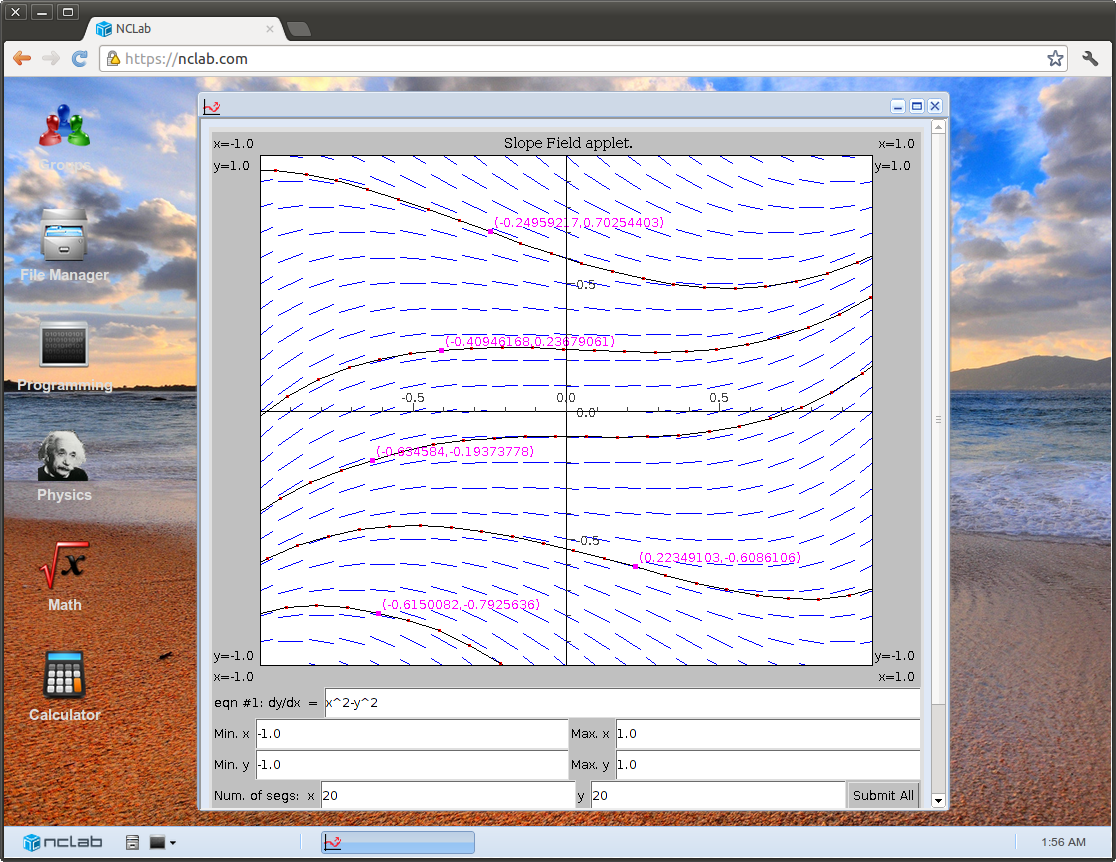
\includegraphics[width=\textwidth]{img/jode1.png}
\end{center}
%\vspace{-2mm}
\caption{Slope fields with JODE.}
\label{fig:jode1}
\end{figure}


\subsection{PDE}

The Partial Differential Equations (PDE) section contains a Finite Element Analysis (FEA)
application for solving general linear second-order equations with constant coefficients.
Illustrative screenshot is shown below.
\newpage
\begin{figure}[!ht]
\begin{center}
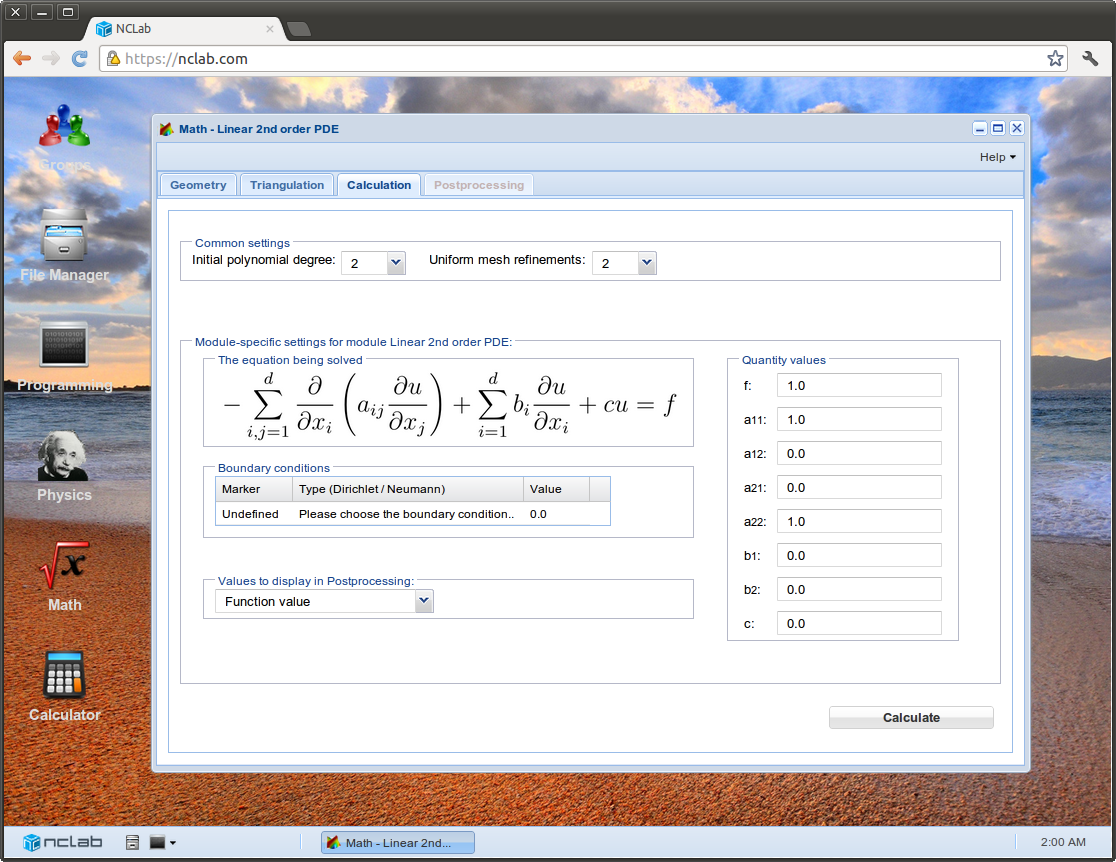
\includegraphics[width=\textwidth]{img/pde1.png}
\end{center}
%\vspace{-2mm}
\caption{Solving linear second-order PDE.}
\label{fig:pde1}
\end{figure}

\section{Solid Modeling (CAD)}

Solid Modeling is the basic principle of CAD systems -- complicated geometries 
and shapes are created using simple objects that can be translated, rotated and scaled. 
One can also create their unions and intersections, and subtract objects 
from each other. NCLab provides Solid Modeling via PLaSM (Programming Language for Solid 
Modeling). 

Professional CAD systems such as SolidWorks or AutoCAD are aimed at maximizing the engineer's
productivity. Therefore, their functionality is highly automated. In contrast to them, PLaSM 
is a scripting language that allows the user to gain a better insight into the underlying 
geometrical operations, as well as create parameter-dependent designs. 
For illustration, the following short script renders a metal cube:
\begin{verbatim}
from pyplasm import *
color = [0.9, 0.9, 0.9]
c = CUBE(1.0)
lab.view(c, color)
\end{verbatim}
Fig. \ref{fig:plasm1} shows more advanced models of a 3D gear and 
a temple:

\begin{figure}[!ht]
\begin{center}
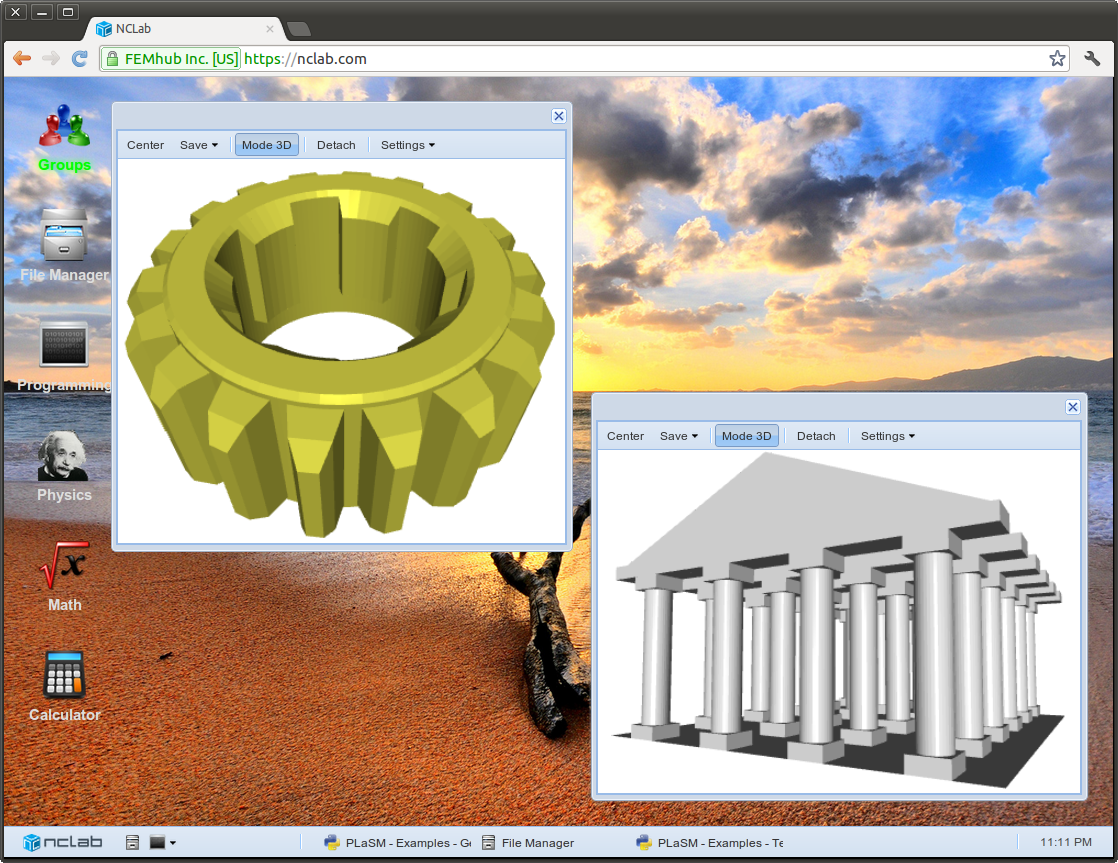
\includegraphics[width=\textwidth]{img/plasm1.png}
\end{center}
%\vspace{-2mm}
\caption{Sample 3D models created with PLaSM.}
\label{fig:plasm1}
\end{figure}
\noindent
To learn more, read the PLaSM tutorial and watch a three-part YouTube video!
\newpage

\section{Review Questions}

\begin{enumerate}
\item What is {\em Cloud}?
\begin{enumerate}
\item[A1] Large pool of interconnected computers.
\item[A2] Local LAN network in an organization or school.
\item[A3] Computer that is equipped with keyboard but not monitor.
\item[A4] Company that manufactures large computer clusters.
\end{enumerate}
\item Name at least one free cloud service.
\begin{enumerate}
\item[A1] Gmail.
\item[A2] United States Postal Service
\item[A3] Fedex
\item[A4] UPS
\end{enumerate}
\item What does the abbreviation {\em SaaS} stand for?
\begin{enumerate}
\item[A1] Simple and always Stable.
\item[A2] Synchronized and automated Service.
\item[A3] Software as a Service.
\item[A4] Super addictive and Sweet.
\end{enumerate}
\item What is WebGL?
\begin{enumerate}
\item[A1] Webinar on Grenade Launchers.
\item[A2] Advanced 3D graphics in the web browser.
\item[A3] Web page of the Girls Life magazine.
\item[A4] Abbreviation for "Good Luck" among web designers.
\end{enumerate}
\item What is the main advantage of GPUs over CPUs?
\begin{enumerate}
\item[A1] GPUs are smaller and lighter than CPUs.
\item[A2] GPUs are cheaper than CPUs.
\item[A3] GPUs provide much more computing power than similarly priced CPUs.
\item[A4] GPUs can operate without electricity.
\end{enumerate}
\item Name one of the most famous fractal sets.
\begin{enumerate}
\item[A1] Mandelbrot.
\item[A2] Zuckerberg.
\item[A3] Heisenberg.
\item[A4] Heidenhain.
\end{enumerate}
\item What makes the Python programming language popular?
\begin{enumerate}
\item[A1] It comes with free compilers.
\item[A2] It does not need any libraries.
\item[A3] C++ is written in Python.
\item[A4] It is easy to use and comes with powerful libraries.
\end{enumerate}
\item What is Javascript?
\begin{enumerate}
\item[A1] Most popular programming language for web development.
\item[A2] Program written in the Java programming language.
\item[A3] Script written in the Java programming language.
\item[A4] The Java runtime environment. 
\end{enumerate}
\item Name the three basic components of Web Design.
\begin{enumerate}
\item[A1] Compiler, interpreter, linker.
\item[A2] HTML, CSS and JS.
\item[A3] Computer, keyboard, mouse.
\item[A4] Firefox, Chrome, Safari.
\end{enumerate}
\item What is Solid Modeling?
\begin{enumerate}
\item[A1] Method to create arbitrary geometries via simple objects.
\item[A2] Computer modeling in Solid Mechanics.
\item[A3] Computer modeling in Solid State Physics.
\item[A4] Modeling with {\em Solid} (a computer modeling software).
\end{enumerate}
\end{enumerate}

\end{document}
